% !TEX root = ../Projektdokumentation.tex
\section{Introduction}
\label{sec:Introduction}

The following documentation outlines the process of the project, which was carried out by the authors
in the framework of their IT specialist education.

\subsection{Project Description}
\label{sec:ProjectDescription}
The purpose of the project was to create and realize an entirely new homepage design for the \textit{In\-dus\-trie\-schu\-le Chemnitz}. For 
that matter the authors analysed in precedent meetings with their teachers and the principal the current state of the school's
 internet presence and defined the frame requirements of the completely new website.

\subsection{Previous Situation}
\label{sec:PreviousSituation}
The previous homepage (see Fig. \ref{fig:pageOld}) was based on a design and technology of the year 2002. Although it was certainly well made for its time
it became obsolete after over one decade.
\begin{figure}[ht]
	\centering
	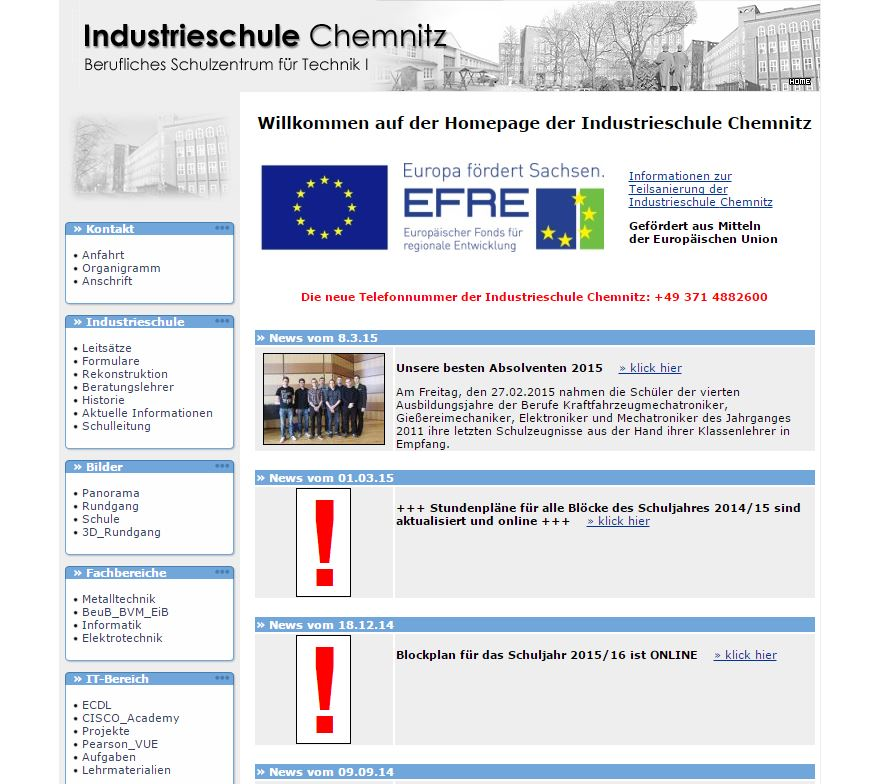
\includegraphics[width=0.80\textwidth]{./Bilder/oldpage.jpg}
	\caption{Main menue of the previous school homepage}
	\label{fig:pageOld}
\end{figure}
The main points of criticism where the missing ease of use, i.e. the old site was not responsive and barrier-free. Also 
the missing content management system complicated administration and updating the page. Furthermore the logical 
menu structure needed revision.

\subsection{Project Objective}
\label{sec:ProjectObjective}
The task of the new homepage was to provide information about the school, its  educational offer and the school life. 
Furthermore it should be applicable to do public relations work, publish news and supply students, 
their parents and the companies of the trainees with materials. Last but not least the website reflects 
the schools media competence for the broad public.\\
It has been decided in advance that the website should be equipped with a stable updateable back-end. 
The appearance of the new website was decided to be plain and functional according to the Flat-Design-Philosophy [\cite{Wik1}]
and fulfil today's requirements for comfort, be responsive and barrier-free.\\
A further challenge was the visualisation of the timetables. The schools timetables where 
generated by an external program and needed to be transformed into \acs{HTML}.
Because of reasons of privacy protection it became necessary to protect the timetables by password. 
In consequence a further requirement of the page was a user management system.